\documentclass[11pt,a4paper]{article}
\usepackage[T 1]{fontenc}
\usepackage[margin=2cm]{geometry}
\usepackage{graphicx,booktabs,amsmath,amssymb,url}
\setlength{\parindent}{0pt}\setlength{\parskip}{4pt}
\setlength{\tabcolsep}{4pt}\setlength{\emergencystretch}{2em}
\begin{document}
\begin{center}\Large DNN Programming Assignment 2\\\normalsize
Viradiya Tushar Rajeshbhai --- 2026aj05073\end{center}
\section*{Problem 1: data, verification and HAR classification}
UCI HAR uses the prescribed nine inertial channels, 128 steps, six activities,
7352 source-training windows and 2947 official test windows. The 21 source-training
subjects and nine test subjects are disjoint. For each seed 0/1/2, four training
subjects are selected by the prescribed NumPy choice for validation. Channel
normalization uses only the remaining training subjects. Figure 1 shows the splits;
Figure 2 shows the validation-selected confusion matrix.
All classifiers use last-state classification, $h=64$, one recurrent layer,
Adam $10^{-3}$, batch 128, ten epochs and norm-1 clipping. Validation macro-F 1
selects checkpoints; reported spreads are sample standard deviations.

The scratch cells match library outputs within $10^{-5}$; assert cells also verify
backward gradients and nonzero initial states. For $g=1,4,3$ gates, the single-bias
count is $gh(d+h+1)$ and PyTorch's two-bias count is $gh(d+h+2)$.
At $d=9,h=64$, RNN/LSTM/GRU counts are 4736/18944/14208 versus
4800/19200/14400. Classifier heads add $6h+6$.
\begin{center}\textbf{Table 1. HAR: three seeds; GTX 1650 training time}\par\smallskip
\begin{tabular}{lllll}\toprule
Model & Acc. (\%) & Macro-F 1 & Params & s/epoch\\\midrule
GRU & 88.0783 $\pm$ 0.6369 & 0.8807 $\pm$ 0.0063 & 14790 & 0.213\\
LSTM & 87.5014 $\pm$ 0.4243 & 0.8750 $\pm$ 0.0046 & 19590 & 0.208\\
RNN & 72.4579 $\pm$ 1.0483 & 0.7159 $\pm$ 0.0085 & 5190 & 0.126\\
\bottomrule\end{tabular}\end{center}
\begin{center}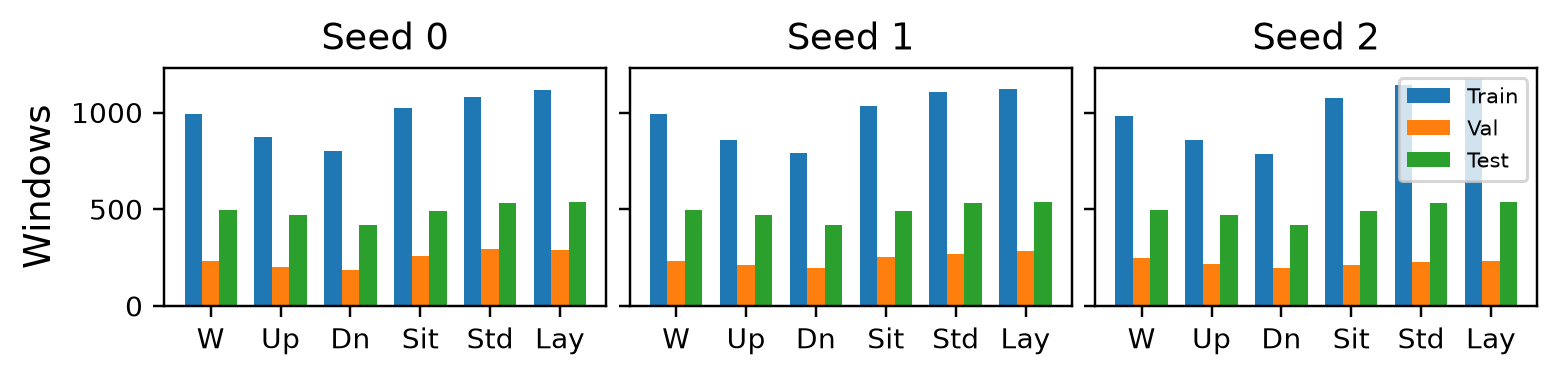
\includegraphics[width=\linewidth,height=2.6cm,keepaspectratio]{problem1/figures/report_class-balance.png}\par Figure 1. Class balance by subject split and official test set.\end{center}
\begin{center}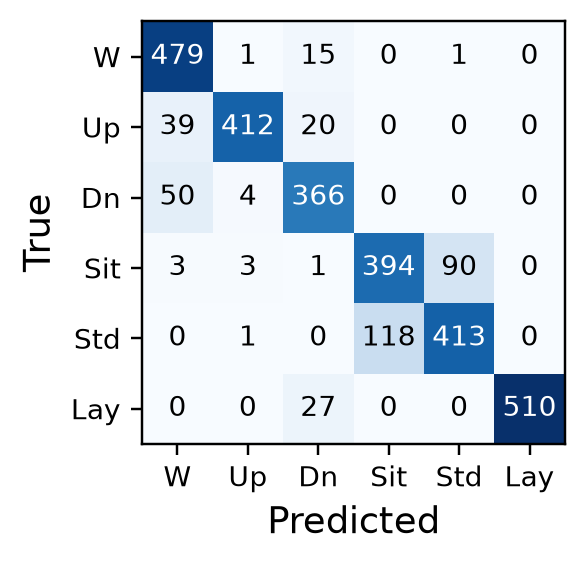
\includegraphics[width=\linewidth,height=3.6cm,keepaspectratio]{problem1/figures/report_confusion.png}\par Figure 2. Validation-selected GRU, seed 2, epoch 9. Table 1 compares all architectures.\end{center}
\newpage
\section*{Problem 1: adding, width and individual ablation}
The prescribed adding generator uses two markers, one per half; assertions check
marker counts and exact target sums. Each length uses 10000/1000/1000 examples
with data seeds 0/1/2. All models use $h=64$, Adam $10^{-3}$, batch 128,
five epochs and clipping 1, with three model seeds. Validation MSE selects weights.
The theoretical constant-1 baseline is $1/6$; Table 2 uses the measured baseline.
Solved means test MSE below 0.05; Figure 3 contains length and learning curves.
\begin{center}\textbf{Table 2. Adding MSE; solved R/L/G counts out of three}\par\smallskip
\begin{tabular}{llllll}\toprule
T & RNN & LSTM & GRU & Constant 1 & Solved\\\midrule
50 & 0.1743 $\pm$ 0.0005 & 0.1743 $\pm$ 0.0003 & 0.1717 $\pm$ 0.0025 & 0.1754 & 0/0/0\\
100 & 0.1700 $\pm$ 0.0005 & 0.1700 $\pm$ 0.0008 & 0.1693 $\pm$ 0.0008 & 0.1697 & 0/0/0\\
200 & 0.1686 $\pm$ 0.0008 & 0.1684 $\pm$ 0.0005 & 0.1685 $\pm$ 0.0003 & 0.1679 & 0/0/0\\
400 & 0.1545 $\pm$ 0.0003 & 0.1538 $\pm$ 0.0005 & 0.1535 $\pm$ 0.0003 & 0.1527 & 0/0/0\\
\bottomrule\end{tabular}\end{center}
\begin{center}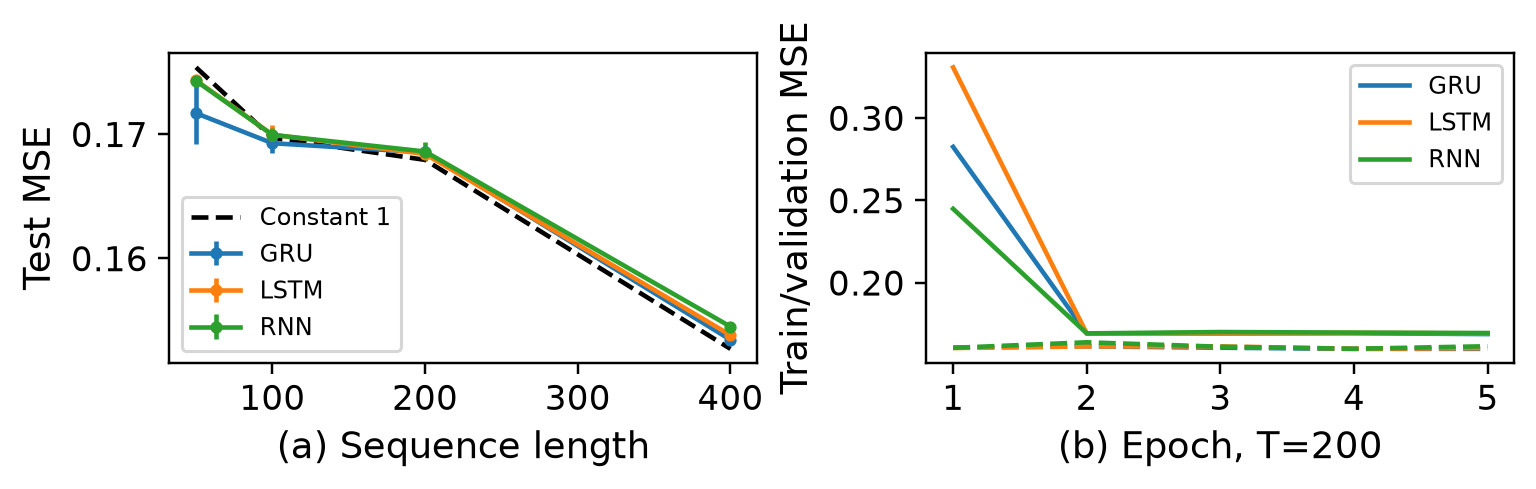
\includegraphics[width=\linewidth,height=2.8cm,keepaspectratio]{problem1/figures/report_adding.png}\par Figure 3. Test MSE against length; T=200 train/validation curves.\end{center}
The hidden-size sweep keeps the HAR budget fixed (Table 3). ID ends in 3, so the individual experiment compares initial LSTM forget bias 0/1 at T=200 (Table 4); other initial weights and shuffle seeds are paired. Figure 4 shows both studies.
\begin{center}\textbf{Table 3. HAR hidden-size sweep}\par\smallskip
\begin{tabular}{lllll}\toprule
h & LSTM acc. (\%) & Params & GRU acc. (\%) & Params\\\midrule
16 & 76.2697 $\pm$ 6.6941 & 1830 & 78.7694 $\pm$ 2.0219 & 1398\\
32 & 83.8254 $\pm$ 1.8710 & 5702 & 87.3317 $\pm$ 1.1564 & 4326\\
64 & 87.5014 $\pm$ 0.4243 & 19590 & 88.0783 $\pm$ 0.6369 & 14790\\
128 & 87.7276 $\pm$ 0.6798 & 71942 & 88.9492 $\pm$ 0.1930 & 54150\\
\bottomrule\end{tabular}\end{center}
\begin{center}\textbf{Table 4. Forget-bias ablation, three seeds}\par\smallskip
\begin{tabular}{lll}\toprule
Bias & MSE & Solved\\\midrule
0 & 0.1684 $\pm$ 0.0004 & 0/3\\
1 & 0.1685 $\pm$ 0.0004 & 0/3\\
\bottomrule\end{tabular}\end{center}
\begin{center}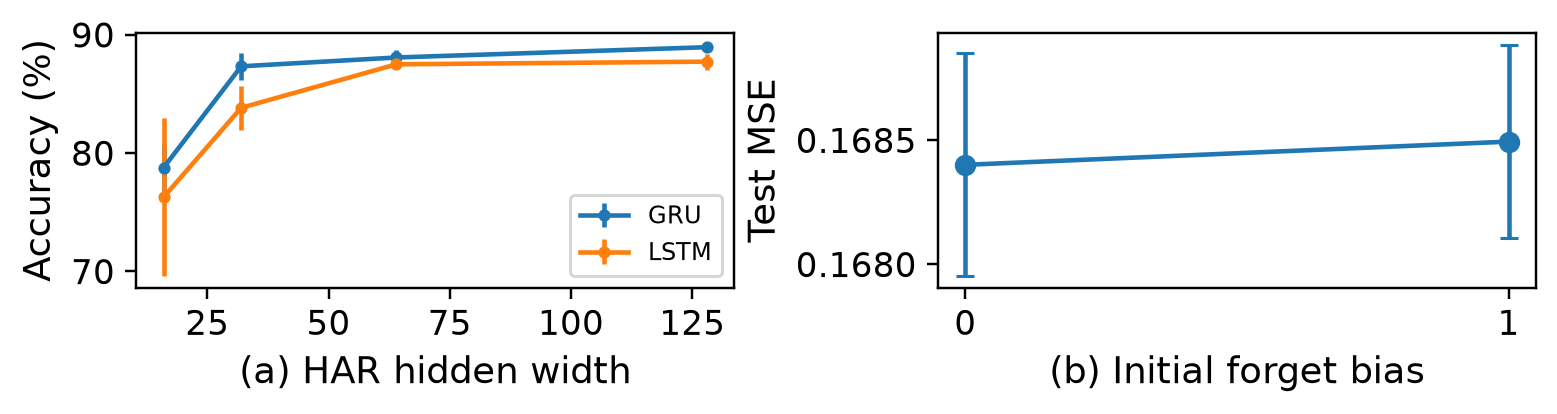
\includegraphics[width=\linewidth,height=2.6cm,keepaspectratio]{problem1/figures/report_sweep-forget.png}\par Figure 4. Hidden-size trade-offs and initial forget-bias comparison.\end{center}
\newpage
\section*{Problem 1: gradient evidence and one-page analysis}
\begin{center}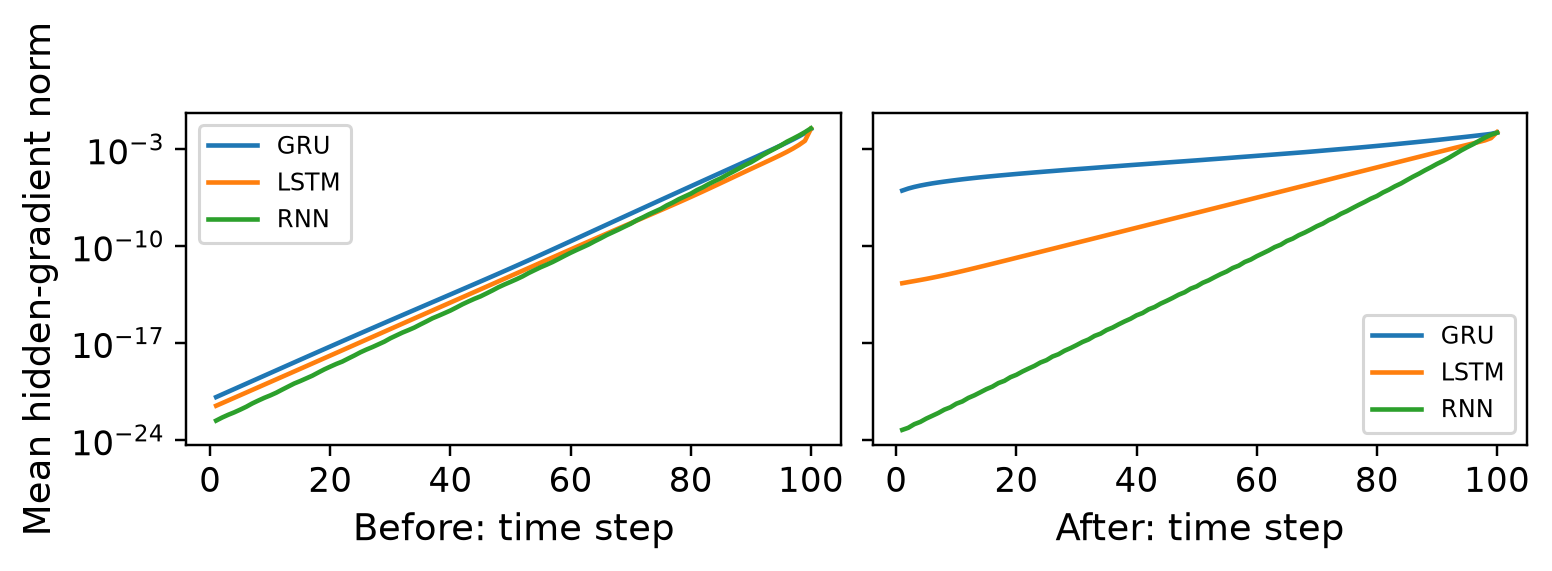
\includegraphics[width=\linewidth,height=4cm,keepaspectratio]{problem1/figures/report_gradients.png}\par Figure 5. Actual hidden-state gradient norms at T=100 before/after training; logarithmic scale, three-seed means.\end{center}
A fixed independent seed 3 probe contains 32 examples. Float 64 custom unrolls
retain each hidden state and verify agreement with library predictions and parameter
gradients. LSTM retains a separate cell-state graph. Small early hidden gradients
indicate weak direct credit assignment to early states, but do not alone measure
all memory carried through an LSTM cell state. Figure 5 should therefore be read
alongside the predictive evidence in Table 2, not as proof that gates solve every task.
RNN: mean post-training first/last hidden-gradient norms are $5.31e-24$/$1.49e-02$. LSTM: mean post-training first/last hidden-gradient norms are $2.05e-13$/$1.65e-02$. GRU: mean post-training first/last hidden-gradient norms are $9.96e-07$/$1.54e-02$. 

Table 2 records 0/36 solved runs at the fixed five-epoch budget. Failure near the constant baseline indicates little useful marker-dependent prediction. It does not establish that the architecture cannot solve the task with another budget. Long sequences increase the credit-assignment distance and computation; three seeds expose instability rather than hiding failed runs.

\begin{center}\textbf{Table 5. T=50 diagnostics on CPU; no test-set evaluation}\par\smallskip
\begin{tabular}{llll}\toprule
Model & Train 32 MSE & Val,5 epochs & Val,25 epochs\\\midrule
RNN & 0.00000 & 0.16681 & 0.16463\\
LSTM & 0.01598 & 0.16587 & 0.01327\\
GRU & 0.00187 & 0.16301 & 0.00189\\
\bottomrule\end{tabular}\end{center}
Table 5 separates fitting 32 examples from generalizing to independent validation
examples. These longer diagnostics support only a limited duration diagnosis at T=50;
they cannot be substituted for the prescribed test grid or claimed as T=400 success.
Table 4 evaluates one paired initialization change rather than a new architecture.
The cell retention factor can improve the early optimization path, but its effect
must be judged from validation-selected test results and seed spread.
For a wearable prototype I would start with GRU, selected by the highest mean validation F 1 (0.9075), then consider the smaller widths in Table 3 if memory is constrained. Its mean test accuracy is 88.08 percent and it has 14790 parameters. Table 1 supplies the measured training-cost trade-off; these GPU training times are not wearable inference latency or energy measurements. Deployment still needs on-device power, latency and accuracy validation.
\newpage
\section*{Problem 2: scratch Transformer and HAR encoder}
Attention is $A=\mathrm{softmax}(QK^T/\sqrt{d_k}+M)$, $O=AV$.
Assertions verify row sums, shapes, zero future weights, gradients and agreement
with PyTorch SDPA within $10^{-5}$. Framework attention/encoder layers are used
only in tests. Fully masked rows are rejected. A nonuniform hand example substitutes
for the absent instructor fixture: $Q=[(1,0);(0,1);(1,1)]$,
$K=[(1,0);(0,1);(1,-1)]$, $V=[(1,0);(0,2);(3,4)]$.
For $a=1/\sqrt 2$, score rows are $(a,0,a),(0,a,-a),(a,a,0)$.
Exponentiate and divide each row by its sum; outputs are
$(1.6044,2.0000),(0.7041,1.7121),(0.9944,1.5933)$, agreeing with code.

Q/K/V/O projections reshape into heads. Pre-LayerNorm blocks use residuals,
ReLU FFN width$4d$ and dropout. Sinusoidal positions use
$PE_{p,2i}=\sin(p/10000^{2i/d})$ and cosine for odd components.
Matrix weights per block are $4d^2+2dd_{ff}$:196608 at $d=128,d_{ff}=512$.
Biases and LayerNorm add $13d=1664$, total 198272, checked by summing parameters.
For the HAR encoder, $d=64$:16384+32768=49152 weights, plus 832 gives 49984.

TaskA uses 8-step patches, a CLS token, $d=64$, two blocks/four heads,
dropout 0.1, batch 128 and ten epochs under the same subject splits. Table 6 and
Figure 6 compare no, sinusoidal and learned positions. Recurrent baselines are in
Table 1; patching, dropout and parameter counts confound architecture-only conclusions.
\begin{center}\textbf{Table 6. HAR encoder, three seeds}\par\smallskip
\begin{tabular}{lllll}\toprule
Position & Acc. (\%) & Macro-F 1 & Params & s/epoch\\\midrule
learned & 91.5847 $\pm$ 2.0396 & 0.9159 $\pm$ 0.0201 & 106310 & 0.269\\
none & 89.5374 $\pm$ 0.7666 & 0.8945 $\pm$ 0.0076 & 105222 & 0.274\\
sinusoidal & 90.3970 $\pm$ 1.1095 & 0.9044 $\pm$ 0.0118 & 105222 & 0.270\\
\bottomrule\end{tabular}\end{center}
\begin{center}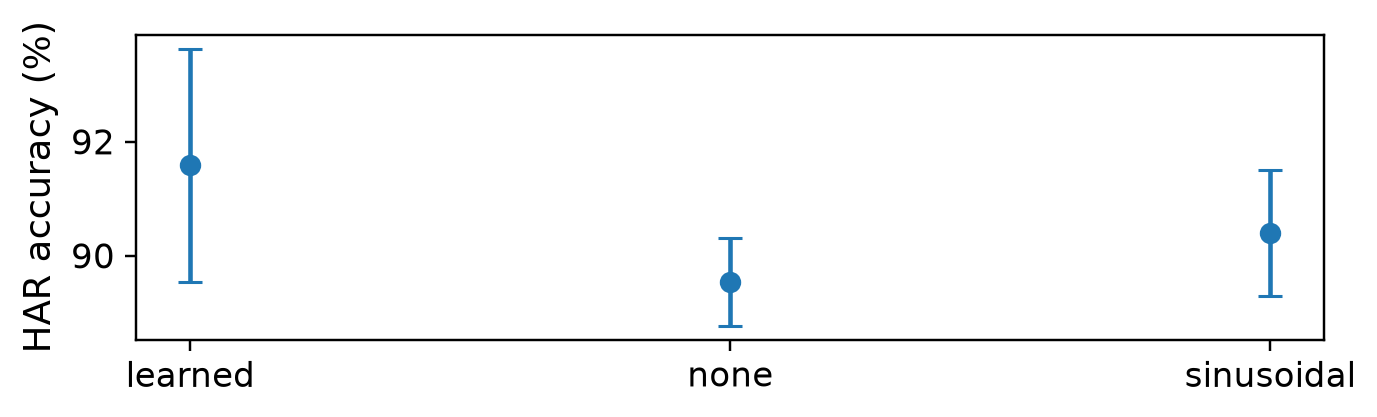
\includegraphics[width=\linewidth,height=3.3cm,keepaspectratio]{problem2/figures/report_positions.png}\par Figure 6. Position ablation; error bars are sample standard deviations.\end{center}
Removing positions makes attention invariant to permutations of whole patches,
verified by reversing patch order. It does not remove order within each flattened
8-step patch. Thus a strong no-position result would not prove temporal order irrelevant.
Sizes/seeds are disclosed assumptions where the variant table is missing.
\newpage
\section*{Problem 2: causal language model and ablations}
Tiny Shakespeare uses its full 65-character vocabulary; the first 90 percent
trains and last 10 percent validates, without shuffled text. The standard GPU model
uses $d=128$, four layers, context 128, four heads, batch 64, dropout 0.1,
Adam $10^{-3}$ and five epochs. Heads 1/4/8 and mask removal have matched budgets.
Four additional five-epoch continuations reset Adam consistently from each selected
baseline. This deliberate restart protocol does not isolate duration from restart effects.
\begin{center}\textbf{Table 7. LM validation; BPC = nats / ln 2}\par\smallskip
\begin{tabular}{lllll}\toprule
Heads & Mask & Base nats & Continued nats & BPC\\\midrule
4 & causal & 1.9093 & 1.7444 & 2.5167\\
1 & causal & 1.8971 & 1.7538 & 2.5302\\
8 & causal & 1.9226 & 1.7547 & 2.5315\\
4 & unmasked & 0.0285 & 0.0210 & 0.0303\\
\bottomrule\end{tabular}\end{center}
\begin{center}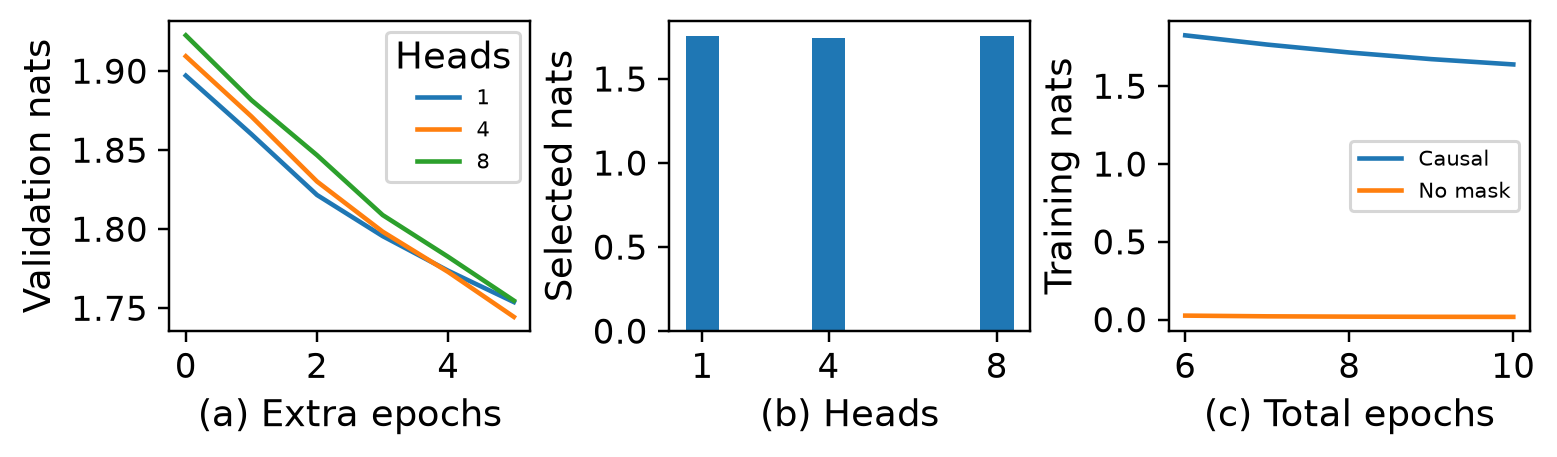
\includegraphics[width=\linewidth,height=4cm,keepaspectratio]{problem2/figures/report_lm-continued.png}\par Figure 7. Validation learning, head ablation and mask-removal training loss.\end{center}
Uniform prediction costs $\ln 65=4.17439$ nats. Table 7 and Figure 7 provide
learning evidence; one seed does not establish a reliable head-count ranking.
Unmasked training exposes the next-character target through future input tokens:
its validation loss is contaminated and is not autoregressive quality. Causal-prefix
invariance and an unmasked counterexample are tested on the trained weights.
The primary LM is the continued four-head causal checkpoint. All samples contain
500 new characters after \texttt{ROMEO:\textbackslash n}, top-k 20, sampling seed 700.
\begin{center}\textbf{Table 8. Sample diversity: continued main model; unmasked baseline}\par\smallskip
\begin{tabular}{lll}\toprule
Temperature/model & Distinct characters & Empirical entropy\\\midrule
0.2 & 26 & 3.673\\
0.8 & 41 & 4.379\\
1.5 & 47 & 4.687\\
unmasked,0.8 & 1 & -0.000\\
\bottomrule\end{tabular}\end{center}
The baseline unmasked draw at 0.8 has 100.0 percent newlines and 100.0 percent identical adjacent characters (Table 8). Compare this generation evidence with its contaminated validation loss in Table 7.
Table 8 describes individual draws, not model predictive entropy. Temperature 0.2 concentrates probability on likely characters;0.8 permits more variation;1.5 flattens the distribution. Higher character diversity is not evidence of coherent language. At 0.2, repeated `shall` fragments dominate;0.8 contains speaker-like `POMPENEy` but malformed `lannio`;1.5 varies punctuation and case while misspelling `wildrak`. The full labelled samples are in generated\_samples.txt.
\newpage
\section*{Problem 2: attention interpretation and context scaling}
\begin{center}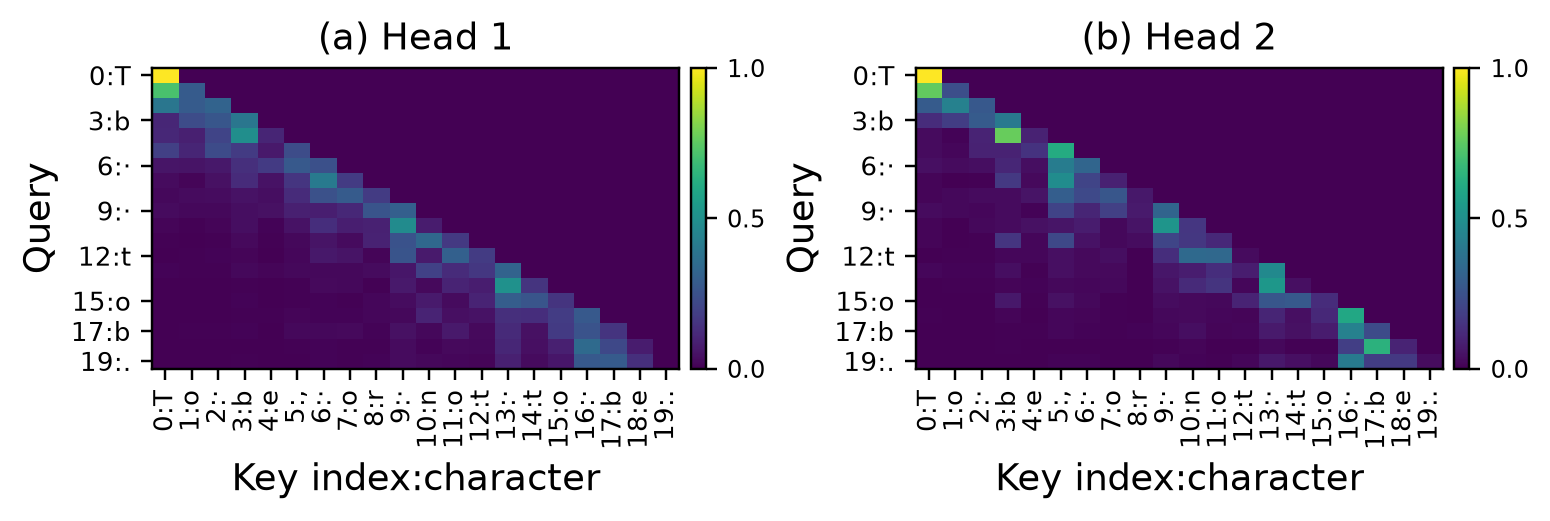
\includegraphics[width=\linewidth,height=4cm,keepaspectratio]{problem2/figures/report_attention-heads.png}\par Figure 8. Baseline first-layer heads 1/2 on ``To be, or not to be. Rows are queries, columns are keys.\end{center}
The mean diagonal masses of the two heads in Figure 8 are 0.2387 and 0.2671. These quantify self-attention for this sentence; off-diagonal weights identify other accessible character positions. Future weights are zero. Different patterns in one sentence do not establish semantic specialization or causal importance.
\begin{center}\textbf{Table 9. GTX 1650 full-model context benchmark}\par\smallskip
\begin{tabular}{lll}\toprule
Context & Time(ms), mean $\pm$ std & Peak tensor MiB\\\midrule
64 & 7.3873 $\pm$ 0.0631 & 16.582\\
128 & 9.3585 $\pm$ 0.0422 & 37.662\\
256 & 17.0292 $\pm$ 0.5549 & 98.960\\
512 & 44.2106 $\pm$ 0.1714 & 309.819\\
\bottomrule\end{tabular}\end{center}
\begin{center}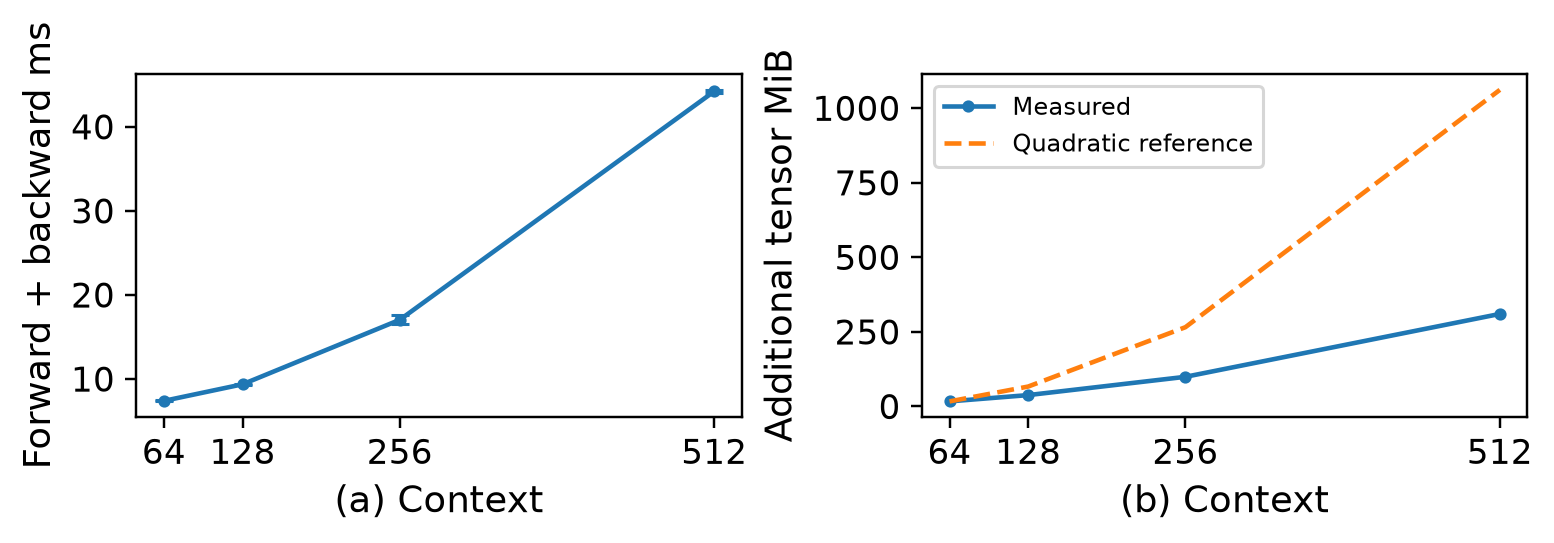
\includegraphics[width=\linewidth,height=3.6cm,keepaspectratio]{problem2/figures/report_context.png}\par Figure 9. Measured time and incremental allocated tensor memory versus context.\end{center}
Table 9/Figure 9 use batch 8, float 32, evaluation-mode forward plus backward, two warmups and five synchronized timing repeats. CUDA peak allocated memory excludes the pre-existing model/input baseline and is not reserved memory. From 64 to 512 tokens, time grows 5.98 times and additional tensor memory 18.68 times. Attention score elements grow 64 times; full-model cost need not exactly follow this ratio because projections and FFNs add linear work.
Execution used a local NVIDIA GeForce GTX 1650 (4 GB). Both complete notebook workflows took 10.00 minutes, excluding environment setup and dataset downloads; this includes tests, evaluation and plots as well as training. Some diagnostics use CPU. The requested runtime is reported for this local GPU; T4 timing was not measured. No bonus is claimed.
\par\textbf{AI-use disclosure.} OpenAI Codex assisted with scratch implementations,
training, testing, execution, plots, analysis and report preparation. The current
assignment permits AI assistance for scratch components.
\newpage
\section*{References}

[1] Course assignment: DNN Programming Assignment--2, RNN, LSTM, GRU and Transformer;
current root DOCX identified by the student. Missing variant table and hand fixture
are handled as explicit assumptions under its missing-information clause.

[2] Vaswani et al., Attention Is All You Need (2017).
\url{https://arxiv.org/abs/1706.03762}. The assignment uses pre-LN, unlike the original post-LN block.

[3] UCI Human Activity Recognition Using Smartphones.
\url{https://archive.ics.uci.edu/dataset/240/human+activity+recognition+using+smartphones}.

[4] Karpathy, Tiny Shakespeare data.
\url{https://github.com/karpathy/char-rnn/tree/master/data/tinyshakespeare}.

[5] PyTorch reference documentation; recurrent and attention modules used for verification.
\url{https://pytorch.org/docs/stable/nn.html}.
\end{document}
